\section{محرمانگی تفاضلی موضعی}
\label{ch:ldp}

در فصل گذشته، مبانی نظری حریم خصوصی متمرکز (\lr{CDP}) و ابزارهای آماری لازم برای تحلیل آن را مرور کردیم. در این فصل، به طور اختصاصی به \textbf{چارچوب محرمانگی تفاضلی موضعی\LTRfootnote{Local Differential Privacy (LDP)}(\LDP)} می‌پردازیم. این مدل، که امروزه در سیستم‌های توزیع‌شده و جمع‌آوری داده‌های بزرگ‌مقیاس کاربرد فراوان دارد، پارادایم اعتماد را از «سرور مرکزی» به «کاربر نهایی» تغییر می‌دهد.

\subsection{مقدمه و گذار از مدل متمرکز}
\label{sec:ldp:intro}

همان‌طور که در بخش \ref{sec:bg:cdp} دیدیم، مدل متمرکز نیازمند وجود یک متصدی مورد اعتماد\LTRfootnote{Trusted Curator} است که به داده‌های خام دسترسی داشته باشد. اگرچه این مدل دقت آماری بالایی را فراهم می‌کند، اما در دنیای واقعی با چالش‌های امنیتی و حقوقی جدی روبروست:
\begin{itemize}
    \item \textbf{نقطه شکست مرکزی\LTRfootnote{Single Point of Failure}:} سرور مرکزی هدف جذابی برای مهاجمان است. نشت اطلاعات از سرور (چه بر اثر هک و چه بر اثر خطای انسانی) حریم خصوصی تمام کاربران را به خطر می‌اندازد.
    \item \textbf{عدم اعتماد کاربران:} در بسیاری از کاربردها (مانند جمع‌آوری داده‌های پزشکی یا تاریخچه مرورگر)، کاربران تمایلی ندارند داده‌های حساس خود را حتی به یک سرور «مطمئن» بسپارند.
\end{itemize}

در پاسخ به این چالش‌ها، مدل محرمانگی تفاضلی موضعی مطرح شد. در \LDP، فرآیند خصوصی‌سازی (افزودن نویز) به سمت کلاینت (کاربر) منتقل می‌شود. به این معنا که داده‌ها \textit{قبل} از ترک دستگاه کاربر، نویزدار می‌شوند و سرور تنها به داده‌های بی‌نام و نویزدار دسترسی دارد (شکل \ref{fig:ldp-model}).

\begin{figure}[ht]
	\centering
	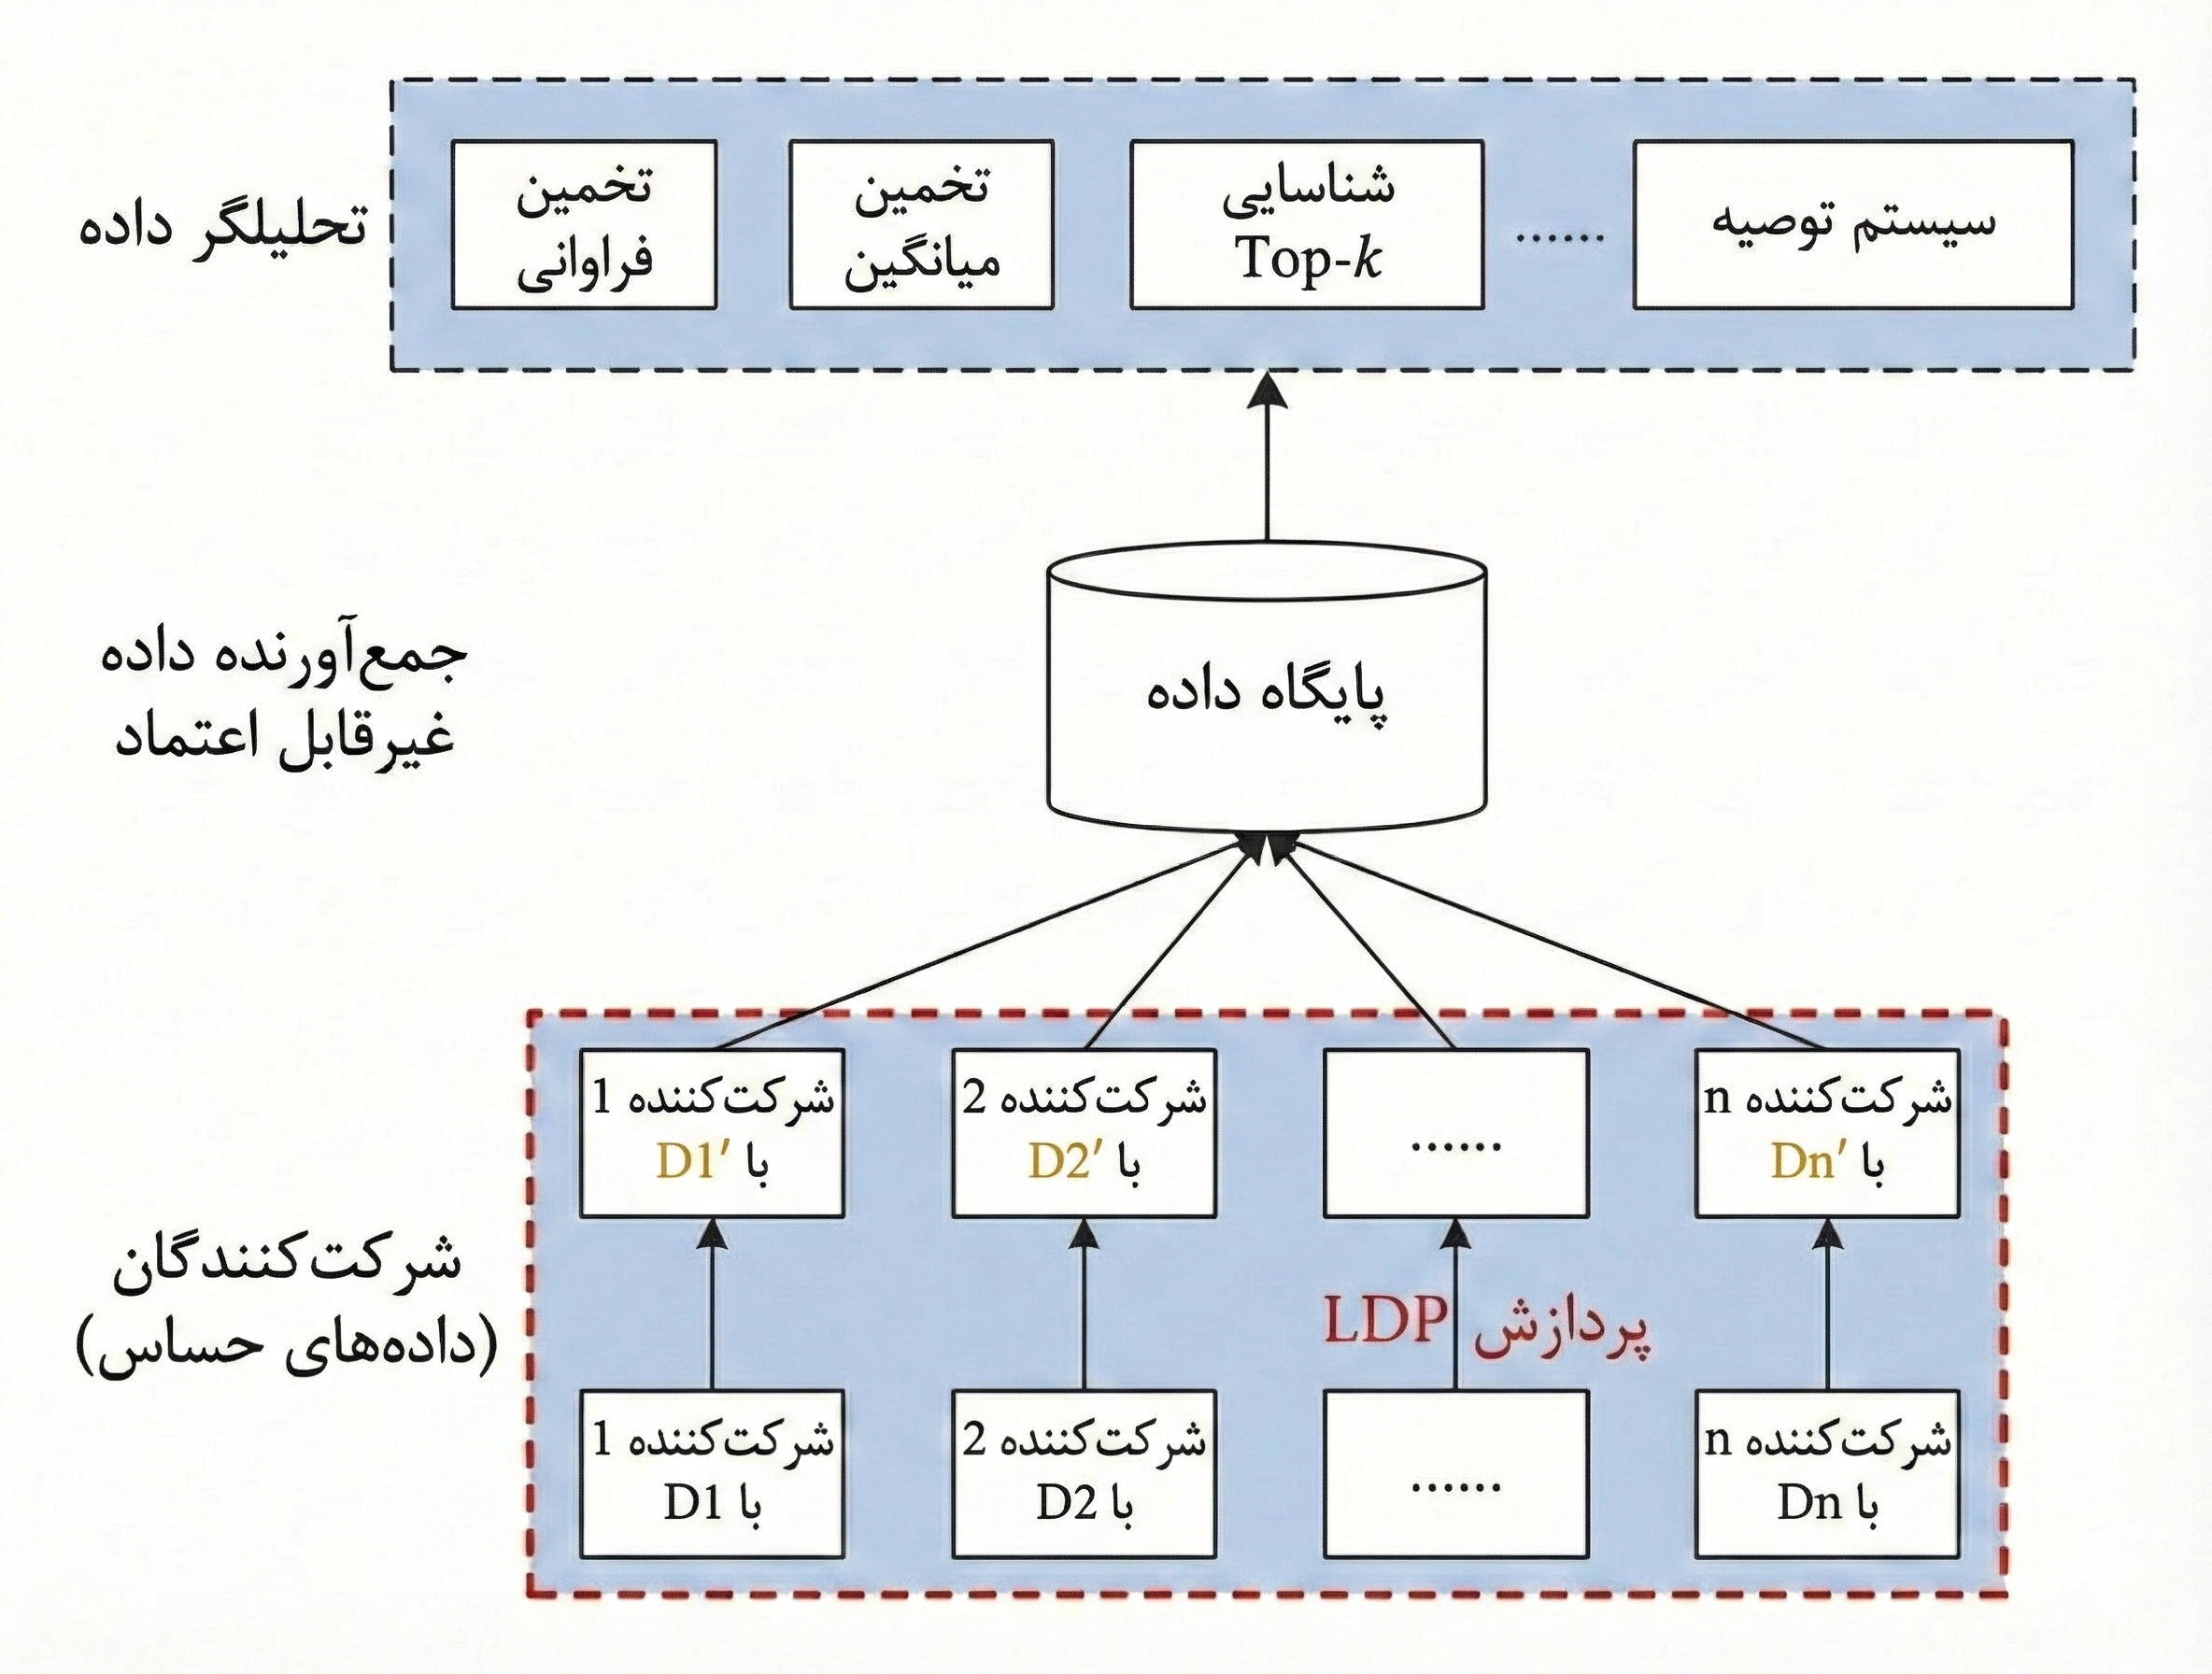
\includegraphics[width=0.7\textwidth]{figs/LDP.png}
	\caption{مدل محرمانگی تفاضلی موضعی (\LDP). نویز به صورت موضعی روی دستگاه کاربر اضافه می‌شود.}
	\label{fig:ldp-model}
\end{figure}

این رویکرد توسط شرکت‌های بزرگ فناوری برای جمع‌آوری داده‌های تله‌متری پذیرفته شده است. برای مثال، گوگل از مکانیزم \lr{RAPPOR} در مرورگر کروم، و اپل و مایکروسافت از روش‌های مشابهی برای جمع‌آوری داده‌های آماری از سیستم‌عامل‌های خود استفاده می‌کنند.

\subsection{تعاریف رسمی و مدل‌های محاسباتی}
\label{sec:ldp:definitions}

در مدل موضعی، ما $n$ کاربر داریم که هر کدام یک داده‌ی خصوصی $X_i$ از دامنه $\Xset$ در اختیار دارند. هر کاربر به طور مستقل یک الگوریتم تصادفی (مکانیزم) را اجرا می‌کند و خروجی $Z_i$ را منتشر می‌کند.

\subsubsection{تعریف \LDP}

هسته‌ی اصلی این مدل، «تصادفی‌ساز موضعی» است.

\begin{تعریف}[تصادفی‌ساز موضعی\LTRfootnote{Local Randomizer}]
یک مکانیزم تصادفی $\mech: \Xset \to \Zset$ را یک تصادفی‌ساز موضعی می‌نامیم که ورودی $x \in \Xset$ را می‌گیرد و خروجی $z \in \Zset$ را بر اساس توزیع احتمال شرطی $Q(z|x)$ تولید می‌کند.
\end{تعریف}

شرط محرمانگی در اینجا تضمین می‌کند که با مشاهده‌ی خروجی $z$، تمایز قائل شدن بین هر دو ورودی اولیه $x$ و $x'$ دشوار باشد. تفاوت کلیدی این تعریف با مدل متمرکز در این است که در \lr{CDP} ما دو پایگاه داده‌ی همسایه را مقایسه می‌کردیم، اما در اینجا هر دو مقدار ورودی ممکن مقایسه می‌شوند.

\begin{تعریف}[$\alpha$-محرمانگی تفاضلی موضعی]
\label{def:alpha-ldp}
یک مکانیزم $\mech$ دارای $\alpha$-محرمانگی تفاضلی موضعی (\LDP) است اگر برای تمام جفت ورودی‌های $x, x' \in \Xset$ و هر زیرمجموعه از خروجی‌ها $\Sset \subseteq \Zset$ داشته باشیم:
\begin{equation}
\label{eq:ldp-def}
\sup_{S} \frac{\Pr[\mech(x) \in \Sset]}{\Pr[\mech(x') \in \Sset]} \le e^{\alpha}
\end{equation}
\end{تعریف}
(نکته: در متون آماری مانند \cite{Duchi2013} معمولاً از پارامتر $\alpha$ به جای $\eps$ برای نمایش بودجه حریم خصوصی موضعی استفاده می‌شود تا تمایز آن با مدل متمرکز مشخص باشد. ما نیز در این فصل و فصول بعدی از این نمادگذاری پیروی می‌کنیم).

این تعریف معادل شرط زیر بر روی واگرایی ماکزیمم ($D_\infty$) بین توزیع‌های شرطی است:
\begin{equation}
\sup_{x, x' \in \Xset} D_\infty(Q(\cdot|x) || Q(\cdot|x')) \le \alpha
\end{equation}

\subsubsection{تعمیم‌ها و خواص}

علاوه بر تعریف استاندارد \LDP (معادله \ref{eq:ldp-def})، دو مفهوم دیگر نیز در تحلیل‌های نظری و طراحی مکانیزم‌ها اهمیت دارند: محرمانگی تقریبی و خاصیت ترکیب.

\begin{تعریف}[$(\alpha, \delta)$-محرمانگی تفاضلی موضعی]
\label{def:approx-ldp}
یک مکانیزم تصادفی $\mech$ دارای محرمانگی تفاضلی موضعی تقریبی یا \LDP[(\al, \del)] است اگر برای هر دو ورودی $x, x' \in \Xset$ و هر زیرمجموعه خروجی $\Sset \subseteq \Zset$ داشته باشیم:
\begin{equation}
\Pr[\mech(x) \in \Sset] \le e^{\alpha} \cdot \Pr[\mech(x') \in \Sset] + \delta
\end{equation}
این تعریف (که در \cite{Wang2020} نیز بررسی شده است)، اجازه‌ی یک احتمال شکست کوچک $\delta$ را می‌دهد. اهمیت نظری این تعریف در آن است که ارتباط مستقیمی با واگرایی $E_\gamma$ (که در فصل قبل معرفی شد) دارد.
\end{تعریف}

\begin{قضیه}[ترکیب ترتیبی\LTRfootnote{Sequential Composition}]
\label{thm:seq-composition}
اگر یک کاربر در $k$ مرحله‌ی مختلف در پروتکل‌های $\mech_1, \dots, \mech_k$ شرکت کند که هر کدام به ترتیب دارای بودجه‌ی حریم خصوصی $\alpha_i$ باشند، آنگاه کل فرآیند دارای محرمانگی تفاضلی موضعی با بودجه‌ی $\sum_{i=1}^k \alpha_i$ خواهد بود.
این خاصیت در تحلیل پروتکل‌های تعاملی (بخش بعد) که در آن خروجی‌های بعدی به خروجی‌های قبلی وابسته هستند، نقش بنیادین دارد.
\end{قضیه}

\subsubsection{پروتکل‌های تعاملی و غیرتعاملی}
\label{sec:ldp:interaction}

یکی از جنبه‌های مهم در تحلیل نرخ‌های مینیماکس (که در فصل بعد به آن می‌پردازیم)، نحوه‌ی تعامل کاربران با سرور است. دوچِی و همکاران \cite{Duchi2013} پروتکل‌های موضعی را به دو دسته تقسیم می‌کنند:

\textbf{۱. پروتکل‌های غیرتعاملی\LTRfootnote{Non-interactive}:}
در این حالت، خروجی هر کاربر $Z_i$ تنها به ورودی خودش $X_i$ وابسته است و مستقل از داده‌ها یا خروجی‌های سایر کاربران تولید می‌شود.
\begin{equation}
Z_i = \mech_i(X_i)
\end{equation}
این مدل ساده‌ترین و رایج‌ترین شکل پیاده‌سازی \LDP است.

\textbf{۲. پروتکل‌های تعاملی (ترتیبی)\LTRfootnote{Sequential/Interactive}:}
در این حالت، مکانیزم کاربر $i$ می‌تواند به خروجی‌های منتشر شده توسط کاربران قبلی ($Z_1, \dots, Z_{i-1}$) وابسته باشد. به عبارت دیگر، کانال ارتباطی $Q_i$ می‌تواند به صورت پویا بر اساس تاریخچه تغییر کند:
\begin{equation}
Z_i \sim Q_i(\cdot | X_i, Z_1, \dots, Z_{i-1})
\end{equation}
این مدل به الگوریتم‌های تطبیقی اجازه می‌دهد تا دقت تخمین را بهبود بخشند. با این حال، همان‌طور که در فصل بعد خواهیم دید، حتی با وجود تعامل، محدودیت‌های بنیادی \f-واگرایی همچنان مانع از کاهش چشمگیر نرخ خطا می‌شوند.
\subsection{مکانیزم‌های پایه در \LDP}
\label{sec:ldp:mechanisms}

در این بخش، مکانیزم‌های بنیادین را معرفی می‌کنیم که برای تحقق محرمانگی تفاضلی موضعی استفاده می‌شوند. این مکانیزم‌ها بلوک‌های سازنده‌ی پروتکل‌های پیچیده‌تر هستند و بسته به نوع داده (دودویی، دسته‌ای یا عددی) و اندازه دامنه انتخاب می‌شوند.

\subsubsection{پاسخ تصادفی دودویی (\lr{RR})}
\label{sec:ldp:rr}

پایه‌ای‌ترین و کلاسیک‌ترین مکانیزم در مدل موضعی، «پاسخ تصادفی»\LTRfootnote{Randomized Response (RR)} است که دهه‌ها پیش از تعریف رسمی \LDP توسط وارنر \cite{warner1965randomized} برای نظرسنجی‌های حساس معرفی شد. فرض کنید دامنه ورودی دودویی باشد ($\Xset = \{0, 1\}$).

مکانیزم $\mech_{RR}$ با ورودی $x \in \{0, 1\}$، خروجی $z \in \{0, 1\}$ را طبق احتمالات زیر تولید می‌کند:
\begin{equation}
\Pr[z = x] = p, \quad \Pr[z \neq x] = 1 - p
\end{equation}
برای اینکه این مکانیزم شرط \LDP را برآورده کند، طبق تعریف \ref{def:alpha-ldp} باید نسبت احتمالات حداکثر $e^\alpha$ باشد:
\begin{equation}
\frac{\Pr[z=1 | x=1]}{\Pr[z=1 | x=0]} = \frac{p}{1-p} \le e^\alpha
\end{equation}
بنابراین، برای دستیابی به کمترین خطا، پارامتر احتمال $p$ به صورت زیر تنظیم می‌شود:
\begin{equation}
p = \frac{e^\alpha}{1+e^\alpha}
\end{equation}
در این حالت، واریانس تخمین‌گر حاصل از این مکانیزم برابر است با:
\begin{equation}
\mathrm{Var}[\hat{x}] = \frac{e^\alpha}{(e^\alpha - 1)^2}
\end{equation}
این رابطه نشان می‌دهد که برای $\alpha$های کوچک، واریانس به سرعت (تقریباً با نرخ $1/\alpha^2$) افزایش می‌یابد که نشان‌دهنده‌ی هزینه بالای حریم خصوصی در دقت تخمین است.

\subsubsection{پاسخ تصادفی تعمیم‌یافته (\lr{GRR})}
\label{sec:ldp:grr}

زمانی که دامنه ورودی شامل $k > 2$ عنصر باشد ($\Xset = \{1, \dots, k\}$)، از نسخه تعمیم‌یافته پاسخ تصادفی\LTRfootnote{Generalized Randomized Response (GRR)} استفاده می‌شود \cite{Kairouz2016}. این روش تعمیم مستقیم \lr{RR} برای دامنه‌های گسسته است.

در این مکانیزم، برای ورودی $x$:
\begin{equation}
\Pr[\mech(x) = z] = 
\begin{cases} 
p & \text{if } \ \ z = x \\
q & \text{if } \ \ z \neq x
\end{cases}
\end{equation}
از آنجا که مجموع احتمالات باید ۱ باشد، داریم $p + (k-1)q = 1$. همچنین شرط \LDP ایجاب می‌کند که $\frac{p}{q} \le e^\alpha$. با حل این دستگاه معادلات، مقادیر بهینه $p$ و $q$ به صورت زیر به دست می‌آیند:
\begin{equation}
p = \frac{e^\alpha}{e^\alpha + k - 1}, \quad q = \frac{1}{e^\alpha + k - 1}
\end{equation}
این مکانیزم برای دامنه‌های کوچک ($k$ کوچک) بسیار کارآمد است و واریانس آن بهینه است. اما با افزایش $k$، دقت آن به شدت کاهش می‌یابد زیرا احتمال گزارش پاسخ صحیح ($p$) با افزایش $k$ کاهش می‌یابد و به سمت صفر میل می‌کند. بنابراین برای دامنه‌های بزرگ (مانند لغات یک دیکشنری)، \lr{GRR} گزینه مناسبی نیست.

\subsubsection{مکانیزم‌های مبتنی بر کدگذاری یگانی (\lr{UE})}
\label{sec:ldp:ue}

برای غلبه بر مشکل کاهش دقت \lr{GRR} در دامنه‌های بزرگ، خانواده‌ای از مکانیزم‌ها تحت عنوان «کدگذاری یگانی»\LTRfootnote{Unary Encoding (UE)} توسعه یافته‌اند. این رویکرد اساس پروتکل مشهور \lr{RAPPOR} گوگل را تشکیل می‌دهد \cite{Wang2020}.

در این روش، فرآیند خصوصی‌سازی طی دو مرحله انجام می‌شود:
\begin{enumerate}
    \item \textbf{کدگذاری \lr{(Encoding)}:} ورودی $x \in \{1, \dots, k\}$ به یک بردار بیتی $v$ به طول $k$ تبدیل می‌شود که تنها در موقعیت $x$ برابر با ۱ و در سایر جاها ۰ است \lr{(One-hot encoding)}.
    \item \textbf{اختلال \lr{(Perturbation)}:} هر بیت این بردار به صورت مستقل با استفاده از یک مکانیزم باینری معکوس می‌شود.
\end{enumerate}

اگر $v_i$ بیت $i$-ام بردار کدگذاری شده باشد، خروجی $z_i$ به صورت زیر تولید می‌شود:
\begin{equation}
\Pr[z_i = 1] = 
\begin{cases} 
p & \text{if } \ \ v_i = 1 \\
q & \text{if } \ \ v_i = 0
\end{cases}
\end{equation}
بر اساس انتخاب مقادیر $p$ و $q$، دو مکانیزم مهم در این خانواده تعریف می‌شوند:

\begin{itemize}
    \item \textbf{کدگذاری یگانی متقارن (\lr{SUE}):}
    که به آن \lr{Basic RAPPOR} نیز گفته می‌شود. در این حالت، احتمالات تغییر بیت به گونه‌ای انتخاب می‌شوند که مکانیزم متقارن باشد ($p + q = 1$). مقادیر بهینه عبارتند از:
    \begin{equation}
    p = \frac{e^{\alpha/2}}{e^{\alpha/2} + 1}, \quad q = \frac{1}{e^{\alpha/2} + 1}
    \end{equation}
    مزیت SUE این است که واریانس تخمین برای هر آیتم مستقل از تعداد کل آیتم‌ها ($k$) است، اما به دلیل استفاده از نیمی از بودجه حریم خصوصی ($\alpha/2$) برای هر بیت، خطای آن همچنان قابل توجه است.
    
    \item \textbf{کدگذاری یگانی بهینه (\lr{OUE}):}
    وانگ و همکاران \cite{Wang2020} نشان دادند که برای تخمین فراوانی در دامنه‌های بزرگ، نیازی به متقارن بودن مکانیزم نیست. در روش \lr{OUE}\LTRfootnote{Optimized Unary Encoding}، پارامترها به گونه‌ای تنظیم می‌شوند که اطلاعات بیت‌های ۱ (سیگنال اصلی) با بیشترین دقت حفظ شود ($p=1/2$) و نویز روی بیت‌های ۰ (که تعدادشان زیاد است) کنترل شود:
    \begin{equation}
    p = \frac{1}{2}, \quad q = \frac{1}{e^\alpha + 1}
    \end{equation}
    تحلیل‌های نظری و تجربی نشان می‌دهند که \lr{OUE} برای $\alpha$های متوسط و بزرگ، واریانس کمتری نسبت به \lr{GRR} و \lr{SUE} دارد و استاندارد فعلی برای جمع‌آوری داده‌های دسته‌ای بزرگ‌مقیاس است.
\end{itemize}

\subsubsection{مکانیزم لاپلاس موضعی}
\label{sec:ldp:laplace}

برای داده‌های عددی (مثلاً $x \in [-1, 1]$)، استفاده از مکانیزم لاپلاس که در مدل متمرکز محبوب است، در مدل موضعی نیز ممکن است اما با چالش‌هایی همراه است.

حساسیت سراسری ($\Delta$) در مدل موضعی برابر با قطر دامنه است، زیرا هر دو ورودی $x, x' \in \Xset$ باید از نظر مکانیزم غیرقابل تمایز باشند. اگر دامنه ورودی $\Xset = [-1, 1]$ باشد، حساسیت برابر است با:
\begin{equation}
\Delta = \max_{x, x'} |x - x'| = |1 - (-1)| = 2
\end{equation}
بنابراین، مکانیزم لاپلاس موضعی خروجی را به صورت زیر تولید می‌کند:
\begin{equation}
\mech_{Lap}(x) = x + \eta, \quad \eta \sim \mathrm{Lap}\left(\frac{2}{\alpha}\right)
\end{equation}
نکته مهمی که دوچی و همکاران \cite{Duchi2013} به آن اشاره کرده‌اند این است که برخلاف مدل متمرکز، مکانیزم لاپلاس در مدل موضعی برای ابعاد بالا ($d > 1$) \textbf{زیر-بهینه}\LTRfootnote{Sub-optimal} است و نرخ خطای آن بدتر از مکانیزم‌های پیشرفته‌تر (مانند نمونه‌برداری هایپرکیوب) است که در فصل‌های آینده به آن‌ها اشاره خواهیم کرد.

\subsection{چالش سودمندی در مدل موضعی}
\label{sec:ldp:utility}

بهای عدم اعتماد به سرور، کاهش شدید سودمندی\LTRfootnote{Utility} آماری است. از آنجایی که نویز به داده‌ی هر فرد به صورت مستقل اضافه می‌شود، خطای تجمیعی در مدل \LDP بسیار بیش‌تر از مدل متمرکز \lr{CDP} است.

برای رسیدن به سطح دقت مشابه، مدل موضعی معمولاً به تعداد کاربران $n$ بسیار بیشتری نیاز دارد. به طور کلی، در حالی که خطای مکانیزم‌های \lr{CDP} اغلب با $O(1/n)$ کاهش می‌یابد، خطای مکانیزم‌های \LDP معمولاً با $O(1/\sqrt{n})$ کاهش می‌یابد. این کاهش در «اندازه نمونه مؤثر» یکی از موضوعات اصلی است که در فصل آینده با استفاده از ابزارهای \f-واگرایی آن را اثبات خواهیم کرد.